% Options for packages loaded elsewhere
\PassOptionsToPackage{unicode}{hyperref}
\PassOptionsToPackage{hyphens}{url}
%
\documentclass[
]{article}
\usepackage{amsmath,amssymb}
\usepackage{lmodern}
\usepackage{ifxetex,ifluatex}
\ifnum 0\ifxetex 1\fi\ifluatex 1\fi=0 % if pdftex
  \usepackage[T1]{fontenc}
  \usepackage[utf8]{inputenc}
  \usepackage{textcomp} % provide euro and other symbols
\else % if luatex or xetex
  \usepackage{unicode-math}
  \defaultfontfeatures{Scale=MatchLowercase}
  \defaultfontfeatures[\rmfamily]{Ligatures=TeX,Scale=1}
\fi
% Use upquote if available, for straight quotes in verbatim environments
\IfFileExists{upquote.sty}{\usepackage{upquote}}{}
\IfFileExists{microtype.sty}{% use microtype if available
  \usepackage[]{microtype}
  \UseMicrotypeSet[protrusion]{basicmath} % disable protrusion for tt fonts
}{}
\makeatletter
\@ifundefined{KOMAClassName}{% if non-KOMA class
  \IfFileExists{parskip.sty}{%
    \usepackage{parskip}
  }{% else
    \setlength{\parindent}{0pt}
    \setlength{\parskip}{6pt plus 2pt minus 1pt}}
}{% if KOMA class
  \KOMAoptions{parskip=half}}
\makeatother
\usepackage{xcolor}
\IfFileExists{xurl.sty}{\usepackage{xurl}}{} % add URL line breaks if available
\IfFileExists{bookmark.sty}{\usepackage{bookmark}}{\usepackage{hyperref}}
\hypersetup{
  pdftitle={Indeed.com Job Listings Analysis},
  hidelinks,
  pdfcreator={LaTeX via pandoc}}
\urlstyle{same} % disable monospaced font for URLs
\usepackage[margin=1in]{geometry}
\usepackage{graphicx}
\makeatletter
\def\maxwidth{\ifdim\Gin@nat@width>\linewidth\linewidth\else\Gin@nat@width\fi}
\def\maxheight{\ifdim\Gin@nat@height>\textheight\textheight\else\Gin@nat@height\fi}
\makeatother
% Scale images if necessary, so that they will not overflow the page
% margins by default, and it is still possible to overwrite the defaults
% using explicit options in \includegraphics[width, height, ...]{}
\setkeys{Gin}{width=\maxwidth,height=\maxheight,keepaspectratio}
% Set default figure placement to htbp
\makeatletter
\def\fps@figure{htbp}
\makeatother
\setlength{\emergencystretch}{3em} % prevent overfull lines
\providecommand{\tightlist}{%
  \setlength{\itemsep}{0pt}\setlength{\parskip}{0pt}}
\setcounter{secnumdepth}{-\maxdimen} % remove section numbering
\ifluatex
  \usepackage{selnolig}  % disable illegal ligatures
\fi

\title{Indeed.com Job Listings Analysis}
\author{}
\date{\vspace{-2.5em}}

\begin{document}
\maketitle

\hypertarget{section}{%
\subsubsection{}\label{section}}

\hypertarget{introduction}{%
\subsubsection{1. Introduction}\label{introduction}}

The job market is becoming ever more competitive, as a student nowadays
it is harder and harder to land the job of your dreams. COVID-19 has
even made it more challenging for recent graduates to find a fitting
role after graduation. A lot of students complain about the gap between
skills learned during their studies and the actual skills required in
the workfield by companies. This motivates our investigation into Indeed
job vacancy postings to find the skills that are actually required for
different job types.

As Marketing Analytics students, we have both the marketing and
analytical knowledge to succeed in a range of different job types in the
field of marketing. We are interested in what the actual required skills
are for jobs in fields related to our studies. Becoming a data
scientist, data analist or maybe marketeer after our studies will
require different skills and competencies and we would like to know to
which degree we possess these skills and to which extent our study
program effectively prepares us for the job market.

We aspire to find insights to help ourselves as well as our fellow
students in making a choice relating to which skills to improve and
perhaps which skills to forego in order to effectively land their first
job. We aim to conduct our investigation in such a way that the
methodology can be used by anyone for any location in the world and for
any job type on Indeed.com. First of all, for our fellow students, the
keyword and location analysis provide easily interpretable tables to see
which skills are in demand for each roles, together with the best
locations for jobs in the Netherlands. Our entire project is accessible
and usable. The entire workflow can be tweaked to your needs by simply
changing the search term in the scraper. This makes our project valuable
for all job seekers in the world, as they can reproduce our data
scraping and analysis for their specific job wishes.

For this project we decided to narrow down our investigation to the
Netherlands. Three of our four members originate from the Netherlands
and since we and our classmates are all studying at Tilburg University
in the Netherlands right now, job options in the Netherlands are most
relevant to us. Furthermore, we decided to investigate the 4 jobs most
closely related to our master in Marketing Analytics program, being data
scientist, marketeer, data-analist and marketing-analist. By narrowing
down the project by not including too many locations and job searches,
the project workflow will be much smoother and easier to reproduce for
anyone interested in doing so.

\hypertarget{methodology}{%
\subsubsection{2. Methodology}\label{methodology}}

First, we built a web scraper that scrapes the vital information of each
job posting associated with a specific job search. We used the
BeautifulSoup package to collect job ids, job titles, salary, company
name, dates, job summary and salaries if available. Afterwards, we
scraped the job descriptions of the same search results to obtain the
job descriptions of each job posting in a separate dataset by using a
chrome webdriver with Python Selenium. Due to restrictions with
captcha's, we collected multiple small batches of datasets per search
term. In R we merged the data into one big file per search term by
joining the datasets on the unique job id that serves as an identifier
for each separate job advert on Indeed. After merging the files into one
dataset per search term, we cleaned the data by removing duplicate
entries and by cleaning up messy string location names. Location names
such as Amsterdam-Zuid or Velsen-Noord were unwanted because they would
appear as two distinct location in our analysis. Therefore, we wrote a
function that removed all such extra unnecessary information in the
location strings. We added a function that replaced certain unspecified
locations such as Nederland or Randstad into Unknown, signifying that a
job did not specify a specific location.

The final step in the cleaning process was cleaning the salary data. The
salary data was quite sparse and also very messy. Roughly three-quarters
of the data was missing, and for the data available, different measures
were given. Some jobs gave hourly salary rates, whereas other jobs
utilized monthly or yearly income as a salary measure. We made a
function that removes unnecessary character strings in the salary data
and converted all different salary measures into yearly income as a
standard. We calculated yearly income for hourly rates based on 40 hour
work week. We multiplied the hourly rate * 40 * 4 * 12 to get a yearly
income rate based on the hourly wage. For the monthly income, we simply
multiplied with 12 to arrive at a yearly income. Quite a few jobs gave a
salary range instead of a fixed number. For those jobs, we decided to
take the middle of the range. We kept the observations with missing
values for salary in the dataset for the first part of the analysis
because it would significantly reduce the number of observations
otherwise.

\begin{enumerate}
\def\labelenumi{\arabic{enumi}.}
\setcounter{enumi}{2}
\tightlist
\item
  Overview of the data After downloading and merging data we have 4
  datasets in total. 1 dataset per search term for the following search
  terms: Data Scientist, Data Analist, Marketing Analist and Marketeer.
  The following section will provide a short overview of how the
  datasets look like. 3.1 This is how the data\_scientist data set looks
  like: We can see that there are 706 job listings. It contains 13
  columns.
\end{enumerate}

\begin{verbatim}
##  [1] "X"                      "id"                     "title"                 
##  [4] "company"                "location"               "postingdate"           
##  [7] "today"                  "summary"                "salary"                
## [10] "url"                    "description"            "scrapetimesdescription"
## [13] "salary_good"
\end{verbatim}

Here can be observed a summary of data\_scientist.

\begin{verbatim}
##        X              id               title             company         
##  Min.   :  1.0   Length:706         Length:706         Length:706        
##  1st Qu.:177.2   Class :character   Class :character   Class :character  
##  Median :353.5   Mode  :character   Mode  :character   Mode  :character  
##  Mean   :353.5                                                           
##  3rd Qu.:529.8                                                           
##  Max.   :706.0                                                           
##                                                                          
##    location         postingdate           today             summary         
##  Length:706         Length:706         Length:706         Length:706        
##  Class :character   Class :character   Class :character   Class :character  
##  Mode  :character   Mode  :character   Mode  :character   Mode  :character  
##                                                                             
##                                                                             
##                                                                             
##                                                                             
##     salary              url            description       
##  Length:706         Length:706         Length:706        
##  Class :character   Class :character   Class :character  
##  Mode  :character   Mode  :character   Mode  :character  
##                                                          
##                                                          
##                                                          
##                                                          
##  scrapetimesdescription  salary_good     
##  Length:706             Min.   :   4800  
##  Class :character       1st Qu.:  36600  
##  Mode  :character       Median :  49908  
##                         Mean   :  78627  
##                         3rd Qu.:  64800  
##                         Max.   :2098560  
##                         NA's   :557
\end{verbatim}

3.2 This is how the data\_analist data set looks like: We can see that
there are 825 job listings. It contains 13 columns.

\begin{verbatim}
##  [1] "X"                      "id"                     "title"                 
##  [4] "company"                "location"               "postingdate"           
##  [7] "today"                  "summary"                "salary"                
## [10] "url"                    "description"            "scrapetimesdescription"
## [13] "salary_good"
\end{verbatim}

Here can be observed a summary of data\_analist.

\begin{verbatim}
##        X            id               title             company         
##  Min.   :  1   Length:825         Length:825         Length:825        
##  1st Qu.:207   Class :character   Class :character   Class :character  
##  Median :413   Mode  :character   Mode  :character   Mode  :character  
##  Mean   :413                                                           
##  3rd Qu.:619                                                           
##  Max.   :825                                                           
##                                                                        
##    location         postingdate           today             summary         
##  Length:825         Length:825         Length:825         Length:825        
##  Class :character   Class :character   Class :character   Class :character  
##  Mode  :character   Mode  :character   Mode  :character   Mode  :character  
##                                                                             
##                                                                             
##                                                                             
##                                                                             
##     salary              url            description       
##  Length:825         Length:825         Length:825        
##  Class :character   Class :character   Class :character  
##  Mode  :character   Mode  :character   Mode  :character  
##                                                          
##                                                          
##                                                          
##                                                          
##  scrapetimesdescription  salary_good     
##  Length:825             Min.   :   6000  
##  Class :character       1st Qu.:  34506  
##  Mode  :character       Median :  44412  
##                         Mean   :  62025  
##                         3rd Qu.:  54054  
##                         Max.   :3432960  
##                         NA's   :598
\end{verbatim}

3.3 This is how the marketing\_analist data set looks like: We can see
that there are 409 job listings. It contains 13 columns.

\begin{verbatim}
##  [1] "X"                      "id"                     "title"                 
##  [4] "company"                "location"               "postingdate"           
##  [7] "today"                  "summary"                "salary"                
## [10] "url"                    "description"            "scrapetimesdescription"
## [13] "salary_good"
\end{verbatim}

Here can be observed a summary of marketing\_analist.

\begin{verbatim}
##        X            id               title             company         
##  Min.   :  1   Length:409         Length:409         Length:409        
##  1st Qu.:103   Class :character   Class :character   Class :character  
##  Median :205   Mode  :character   Mode  :character   Mode  :character  
##  Mean   :205                                                           
##  3rd Qu.:307                                                           
##  Max.   :409                                                           
##                                                                        
##    location         postingdate           today             summary         
##  Length:409         Length:409         Length:409         Length:409        
##  Class :character   Class :character   Class :character   Class :character  
##  Mode  :character   Mode  :character   Mode  :character   Mode  :character  
##                                                                             
##                                                                             
##                                                                             
##                                                                             
##     salary              url            description       
##  Length:409         Length:409         Length:409        
##  Class :character   Class :character   Class :character  
##  Mode  :character   Mode  :character   Mode  :character  
##                                                          
##                                                          
##                                                          
##                                                          
##  scrapetimesdescription  salary_good   
##  Length:409             Min.   : 4200  
##  Class :character       1st Qu.:36525  
##  Mode  :character       Median :47100  
##                         Mean   :46376  
##                         3rd Qu.:55392  
##                         Max.   :96000  
##                         NA's   :345
\end{verbatim}

\hypertarget{this-is-how-the-marketeer-data-set-looks-like}{%
\subsubsection{3.4 This is how the marketeer data set looks
like:}\label{this-is-how-the-marketeer-data-set-looks-like}}

We can see that there are 872 job listings. It contains 13 columns.

\begin{verbatim}
##  [1] "X"                      "id"                     "title"                 
##  [4] "company"                "location"               "postingdate"           
##  [7] "today"                  "summary"                "salary"                
## [10] "url"                    "description"            "scrapetimesdescription"
## [13] "salary_good"
\end{verbatim}

Here can be observed a summary of marketeer.

\begin{verbatim}
##        X              id               title             company         
##  Min.   :  1.0   Length:872         Length:872         Length:872        
##  1st Qu.:218.8   Class :character   Class :character   Class :character  
##  Median :436.5   Mode  :character   Mode  :character   Mode  :character  
##  Mean   :436.5                                                           
##  3rd Qu.:654.2                                                           
##  Max.   :872.0                                                           
##                                                                          
##    location         postingdate           today             summary         
##  Length:872         Length:872         Length:872         Length:872        
##  Class :character   Class :character   Class :character   Class :character  
##  Mode  :character   Mode  :character   Mode  :character   Mode  :character  
##                                                                             
##                                                                             
##                                                                             
##                                                                             
##     salary              url            description       
##  Length:872         Length:872         Length:872        
##  Class :character   Class :character   Class :character  
##  Mode  :character   Mode  :character   Mode  :character  
##                                                          
##                                                          
##                                                          
##                                                          
##  scrapetimesdescription  salary_good     
##  Length:872             Min.   :   8400  
##  Class :character       1st Qu.:  30600  
##  Mode  :character       Median :  36000  
##                         Mean   :  58519  
##                         3rd Qu.:  42000  
##                         Max.   :2400000  
##                         NA's   :653
\end{verbatim}

\begin{enumerate}
\def\labelenumi{\arabic{enumi}.}
\setcounter{enumi}{3}
\tightlist
\item
  Keyword Analysis
\end{enumerate}

In the following sections we provide the analysis for our research. We
performed 3 types of analysises. 1: skill keyword analysis, in which we
analyze the frequency of occurence for certain technical skills related
to marketing analaytics. 2: location analysis, after knowing the right
skills to pursue for the next job we provide a location analysis in
which we investigate what the top locations for our 4 jobs. 3: salary
analysis, we finish with a short analysis of average salaries for each
job and the best locations salary wise for each job.

4.1 Getting the skill counts for the most important skills in data
science jobs
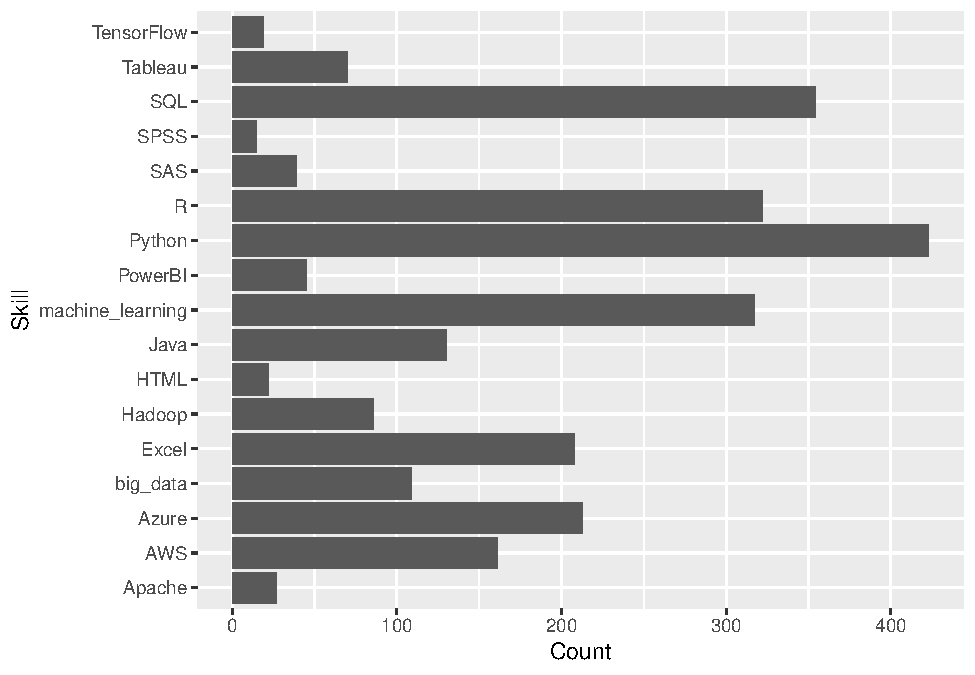
\includegraphics{analysis_files/figure-latex/unnamed-chunk-13-1.pdf}

This is a plot of the core technical skills and their counts in the data
scientist job ads. As we can see, there are 4 clear top skills to learn
to become a data scientist. These include Python, SQL, R and machine
learning, with each having counts over 300. Other important skills seem
to be Java, Excel, Azure and AWS(amazon web services) with each having
counts over 100.

However, counts do not paint the entire picture. Some job ads have
double or even more counts of the same skill within the same
description. To control for this, we also calculate the percentage of
job ads wherein each skill is featured in the description. For example,
if in every second job ad, the skill R is mentioned, it will have a
value of 0.5.\\
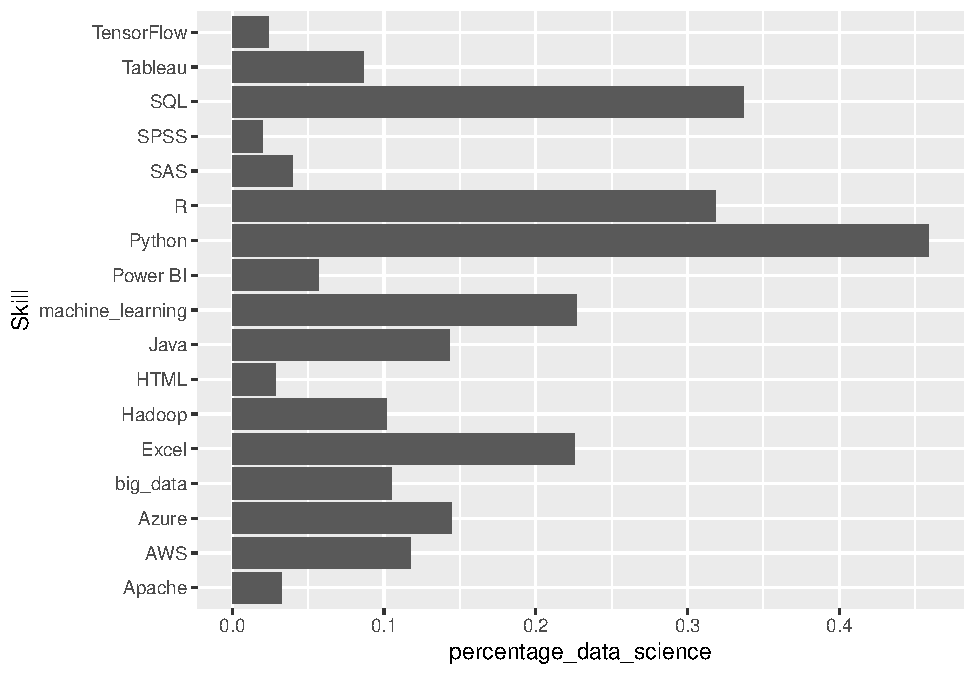
\includegraphics{analysis_files/figure-latex/unnamed-chunk-14-1.pdf} The
percentage plot shows us that the percentage analysis bears quite
similar results to the count analysis. Again Python, R, machine learning
and SQL are the most important skills. However, the difference between
Python and the other skills is bigger in terms of percentage occurrence
than in count. Also in percentage terms, Excel is becoming more
important, catching up with the top 4 skills and being almost equally
important as machine learning.

4.2 Getting the skill counts for the most important skills in
data\_analist jobs

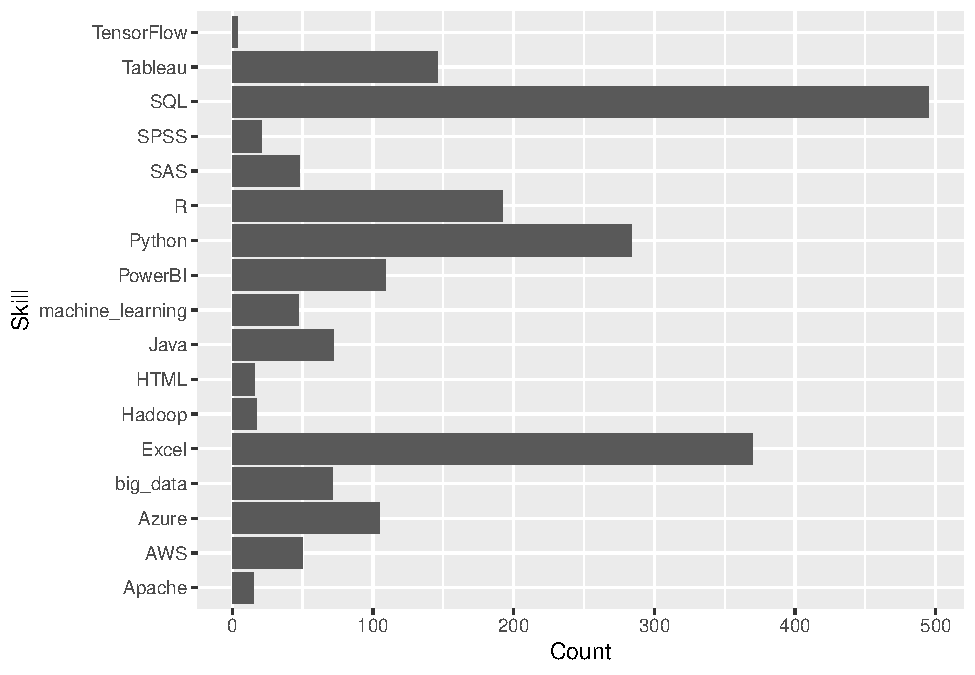
\includegraphics{analysis_files/figure-latex/unnamed-chunk-16-1.pdf}

As we can see, quite a different picture for data analist jobs. The
clear winner is SQL, which approaches the 500 count. After SQL, Excel is
the second most sought after skill with over 350 counts. In 3rd and 4th
come the 2 programming languages Python and R, with Python slightly
edging R in terms of importance. Other important skills inclead Tableau,
Power Bi and Azure.

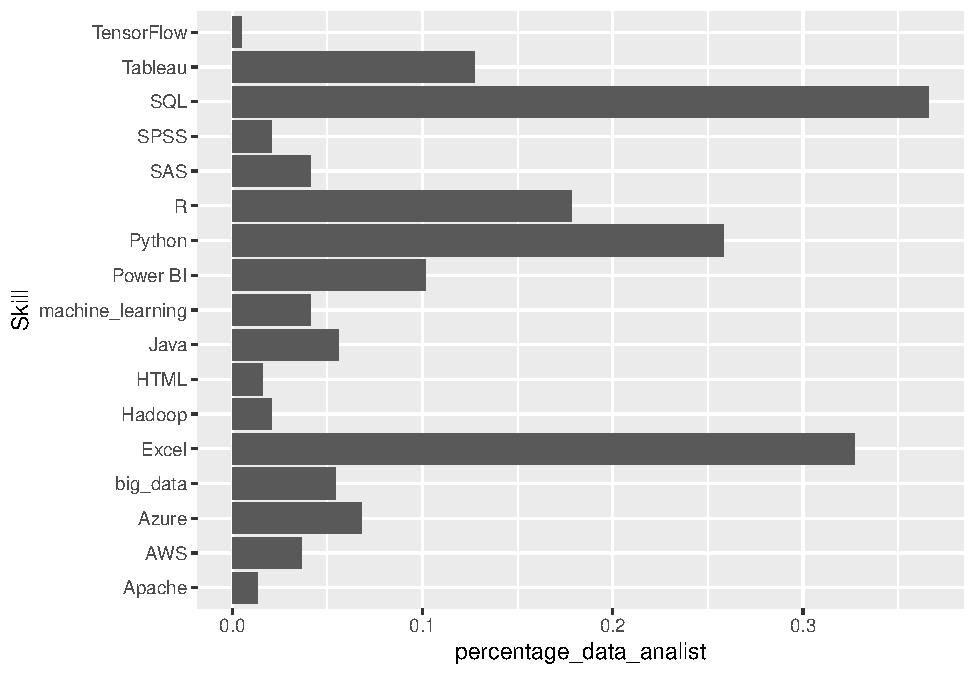
\includegraphics{analysis_files/figure-latex/unnamed-chunk-17-1.pdf}
Again similar results for the percentage analysis. However, the
difference between SQL and Excel is declining, with both being almost
equally important. Also the difference with number 3 Python seems
slightly smaller than in the count analysis. Again other important
skills are R, Power BI and Tableau.

4.3 Getting the skill counts for the most important skills in
marketing\_analist jobs
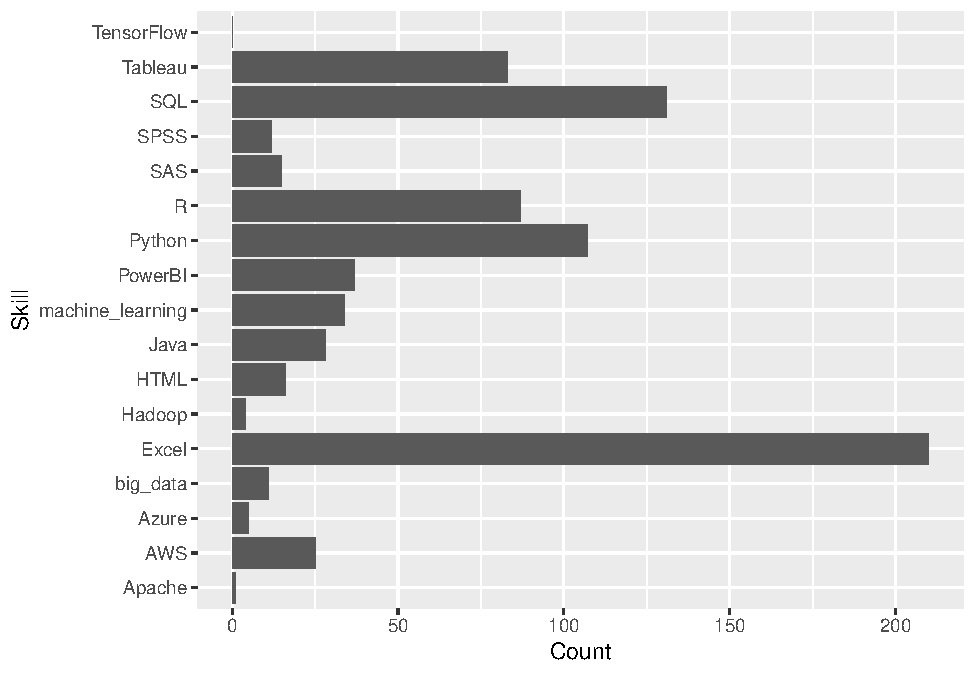
\includegraphics{analysis_files/figure-latex/unnamed-chunk-19-1.pdf}

The clear winner for skills to learn for a marketing analyst is Excel,
being the only skill reaching a count over 200. Other important skills
are SQL, Tableau, R and Python, with all of them being very close to
eachother in terms of relative importance. Then after quite a big gap,
skills such as Power BI, AWS and Azure come, clearly seemingly not that
meaningful to learn as a marketing analist.\\
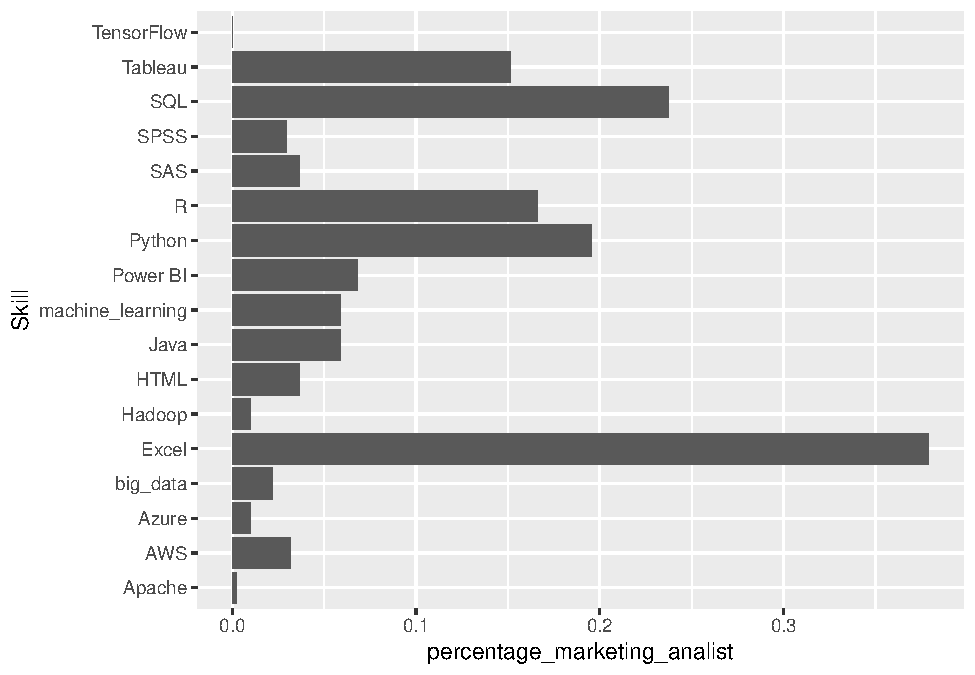
\includegraphics{analysis_files/figure-latex/unnamed-chunk-20-1.pdf}

The Percentage plot shows very similar results to the count plot. Again,
Excel is the clear winner, with mentions in over 1/3 of the job
descriptions. sQL, Python, R and Tableau follow on respected distance
with all being roughly equally relevant for marketing analysts to learn.

4.4 Getting the skill counts for the most important skills in marketeer
jobs
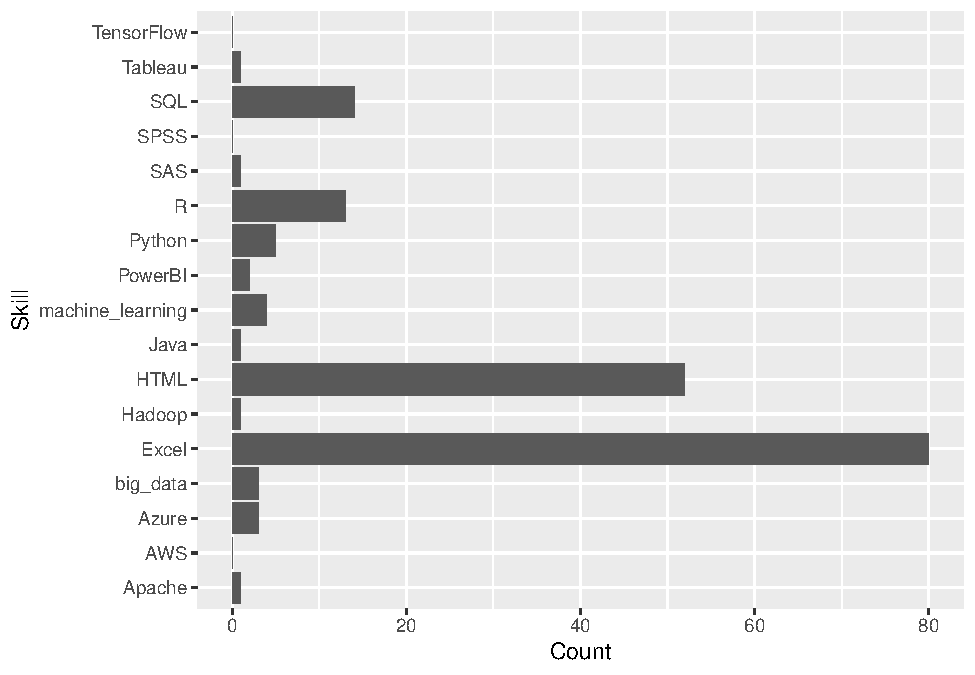
\includegraphics{analysis_files/figure-latex/unnamed-chunk-22-1.pdf} For
Marketeers, it is clear that technical skills are less important than
for the other jobs, which involve more data related tasks. Despite this
fact, Excel is still valuable, being the clear winner for marketeers in
terms of technical skills. 2nd spot is for HTML, which is seen as a
valuable skill for marketeers to have. Other slightly important skills
are R and SQL, with each of the other skills being almost equal to 0 in
terms of occurrences in the job ads for marketeers.

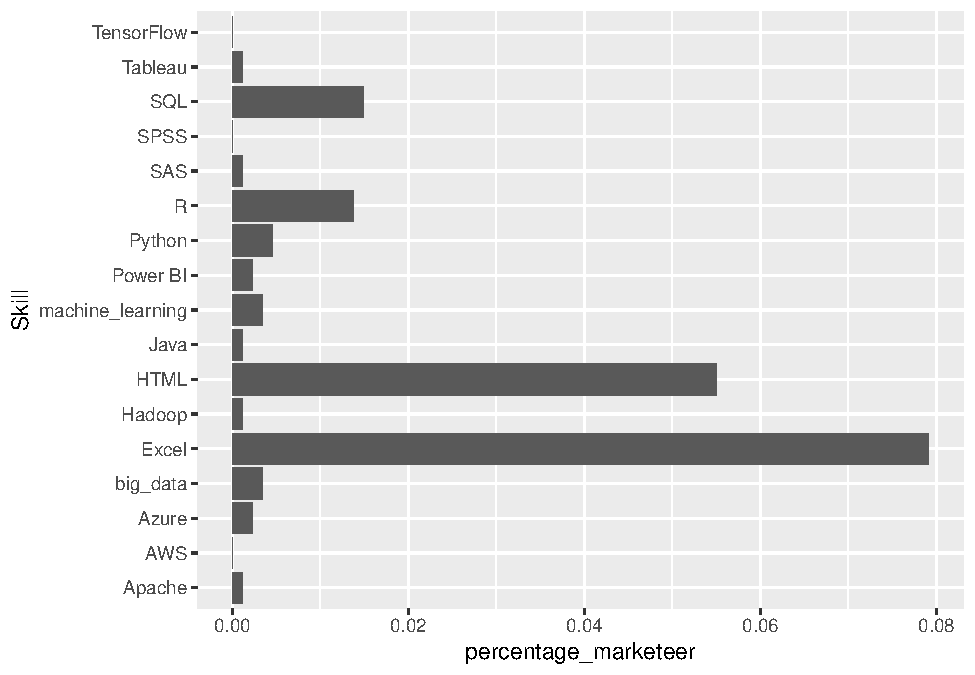
\includegraphics{analysis_files/figure-latex/unnamed-chunk-23-1.pdf}

Similar results in percentage, which show that the technical skills get
mentioned really infrequently in the job advertisements. Excel the
winner in terms of technical skills gets mentioned in only 8 percent of
job ads. Compared with winner skills for other job searches reaching
over 30-40 \%, there is a clear difference in the job requirements for
marketeers.

4.5 Getting insights into comparing the skills from the 4 job titles
Combining the seperate bar charts presented above into one bar graph, to
conveniently compare the skills occurence for our 4 job searches. In the
following section we will provide a comprehensive graph which shows each
skill percentage occurrence for each job next to eachother. In order to
facilitate direct comparison.

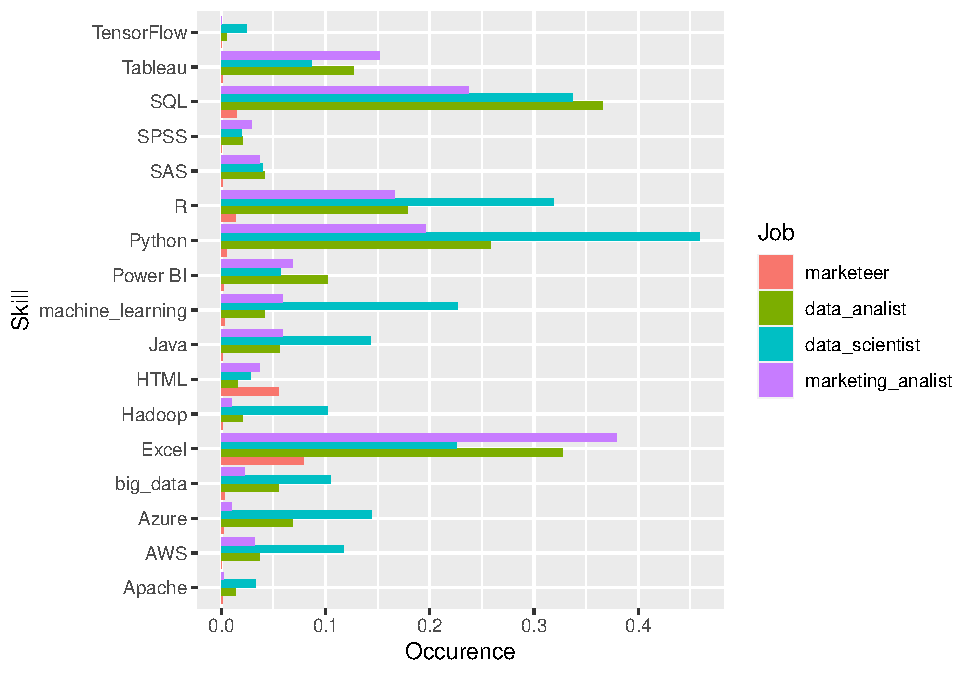
\includegraphics{analysis_files/figure-latex/unnamed-chunk-25-1.pdf} The
top 4 skills in general are Python, R, SQL and Excel. With data
scientist relying heavily on Python whereas fo marketing and data
analysts it might be more fruitful to invest in your SQL skills. There
seems a clear discrepancy between the R and SPSS heavy academic courses
and the actual skills required by companies, more focused on SQL and
Python to perform job tasks. Especially SQL is completely missing from
the Master in Marketing analytics curriculum. Whereas Python is
available in a few courses only.

\begin{enumerate}
\def\labelenumi{\arabic{enumi}.}
\setcounter{enumi}{4}
\tightlist
\item
  Location frequency analysis
\end{enumerate}

5.1 Location frequency data science

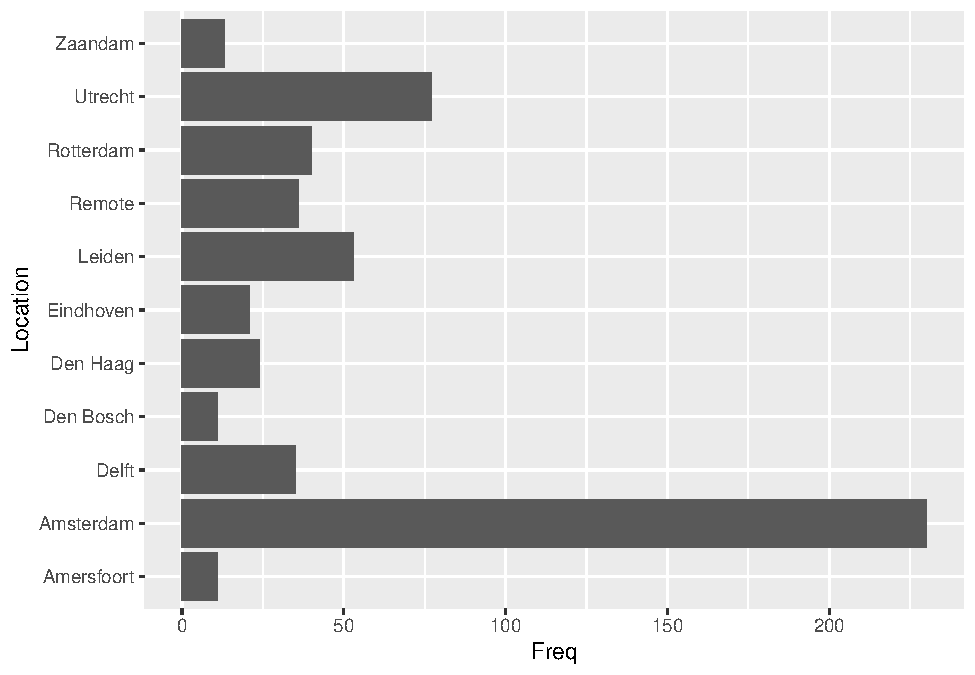
\includegraphics{analysis_files/figure-latex/unnamed-chunk-27-1.pdf}
Amsterdam seems the place to be as a data scientist, with counts over
200, or roughly 1/3 of the entire number of jobs posted being in
Amsterdam. Furthermore, as expected, the randstad features the most in
job ads, with Utrecht, Rotterdam and Leiden coming in high as well.
Outside of the randstad, Noord-Brabant in the form of Eindhoven and Den
Bosch provide a decent number of job opportunities.

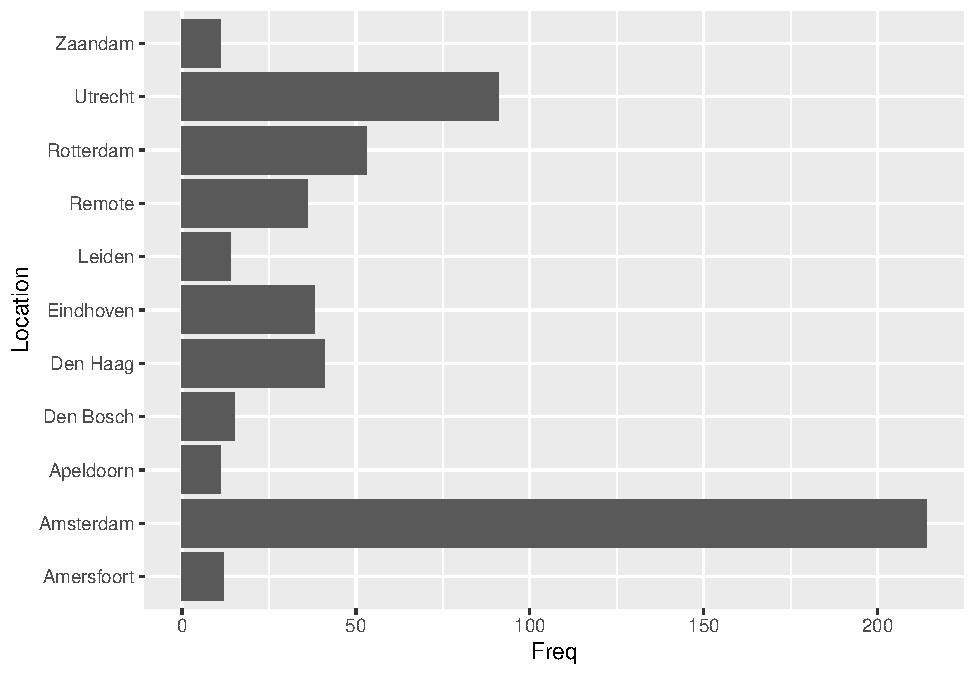
\includegraphics{analysis_files/figure-latex/unnamed-chunk-28-1.pdf} 5.2
Location frequency data analist

For data analysts, the picture is quite similar. Amsterdam again is the
clear winner in terms of number of jobs offered, however, Utrecht seems
relatively more important for data analysts compared to data scientists.
Rotterdam again is number 3, with Den Haag and Eindhoven completing the
top 5 in terms of locations.

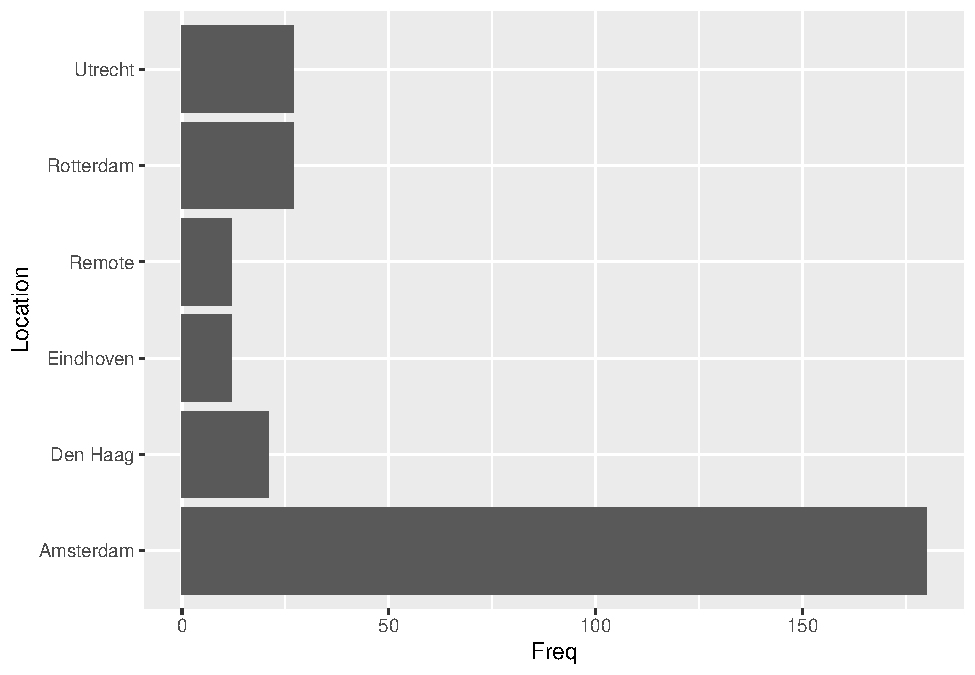
\includegraphics{analysis_files/figure-latex/unnamed-chunk-29-1.pdf} 5.3
Location frequency marketing analist

For Marketing analysts we see the same top 5 as for data analysts.
However, Utrecht, Rotterdam and Den Haag all have almost equal counts of
Job offers and Amsterdam is a way more pronounced winner for Marketing
analysts than for the other jobs scrutinized before.

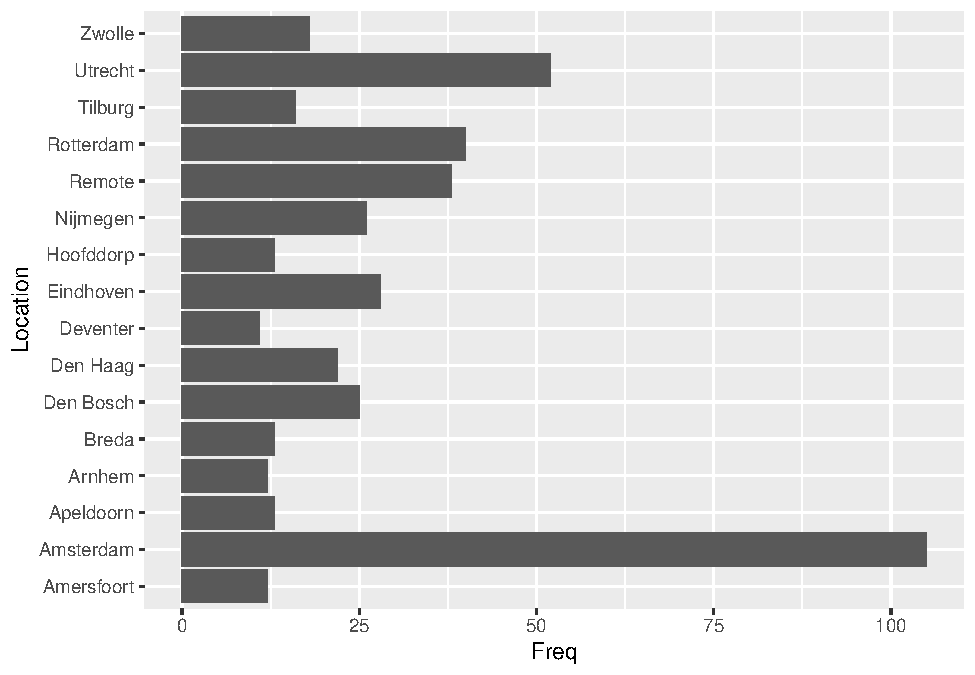
\includegraphics{analysis_files/figure-latex/unnamed-chunk-30-1.pdf} 5.4
Location frequency marketeer

For Marketeers, it seems that there are more opportunities outside of
the randstad available compared to the 3 data related jobs. Cities as
Breda, Arnhem, Deventer and Nijmegen come in quite close to the randstad
cities such as Rotterdam and Utrecht, suggesting that the job
opportunities for marketeers are more evenly spread across the country.

\begin{verbatim}
## Warning in merge.data.frame(location, marketing_analist_location, by =
## "location"): column names 'Var1.x', 'Freq.x', 'Var1.y', 'Freq.y' are duplicated
## in the result
\end{verbatim}

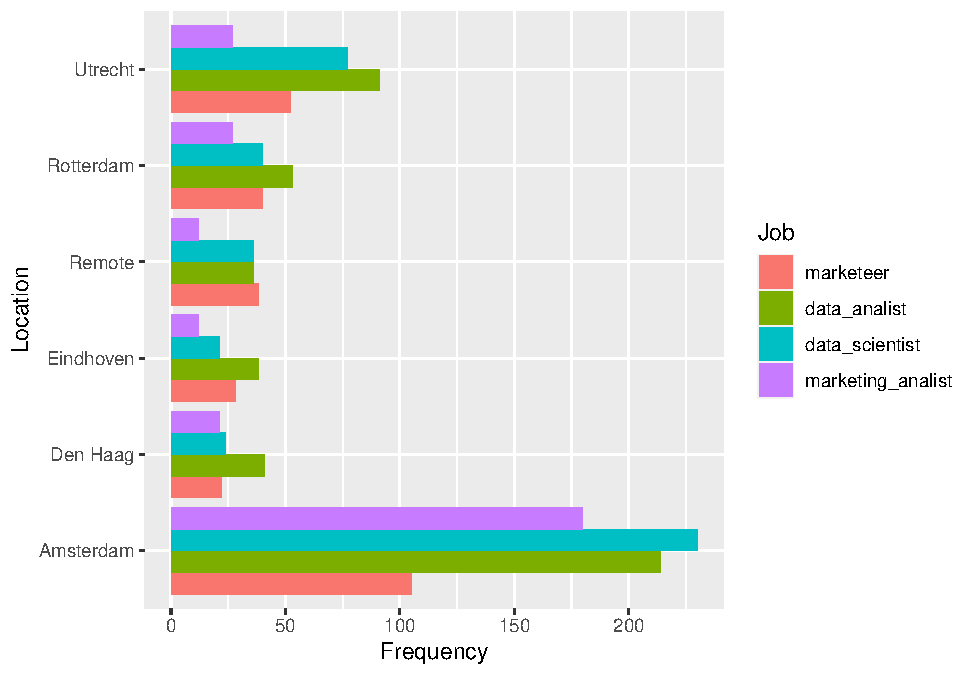
\includegraphics{analysis_files/figure-latex/unnamed-chunk-31-1.pdf} 5.5
Getting insights into comparing the locations of the 4 job titles

This graph show the top 5(plus remote) locations for job ads. As
expected, Amsterdam is the clear winner for each job in terms of number
of job offers, however the difference is less pronounced for marketeer
related jobs than the other 3 jobs. Utrecht comes in 2nd in terms of
number of job fofers whereas Rotterdam, Eindhoven and Den Haag are very
equally ranked.

Now that we know what the most important skills are to learn for our 4
jobs and also what the best cities are to go to, to find a job quickly,
we analyze the best jobs and locations in terms of pay.

\begin{verbatim}
## Warning: Expected 2 pieces. Missing pieces filled with `NA` in 617 rows [1, 2,
## 3, 4, 5, 6, 7, 8, 9, 10, 11, 12, 13, 14, 15, 16, 17, 18, 19, 20, ...].
\end{verbatim}

\begin{verbatim}
## Warning: Expected 2 pieces. Missing pieces filled with `NA` in 671 rows [2, 3,
## 4, 7, 9, 10, 11, 12, 13, 14, 15, 16, 18, 19, 21, 22, 24, 25, 28, 29, ...].
\end{verbatim}

\begin{verbatim}
## Warning: Expected 2 pieces. Missing pieces filled with `NA` in 365 rows [1, 2,
## 3, 4, 5, 6, 7, 9, 10, 11, 13, 14, 15, 16, 17, 18, 19, 20, 22, 23, ...].
\end{verbatim}

\begin{verbatim}
## Warning: Expected 2 pieces. Missing pieces filled with `NA` in 716 rows [1, 2,
## 3, 5, 6, 8, 9, 10, 11, 13, 14, 15, 17, 18, 19, 20, 21, 22, 24, 25, ...].
\end{verbatim}

6 Salary analysis

6.1 mean salaries per job
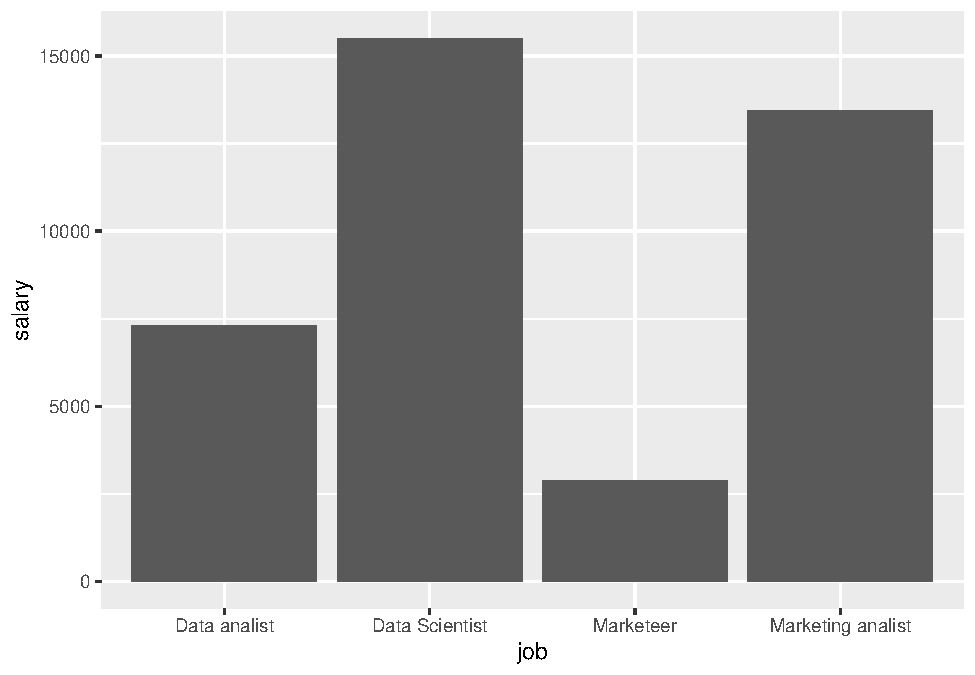
\includegraphics{analysis_files/figure-latex/unnamed-chunk-34-1.pdf}
\includegraphics{analysis_files/figure-latex/unnamed-chunk-34-2.pdf}

\begin{verbatim}
## [1] 4
\end{verbatim}

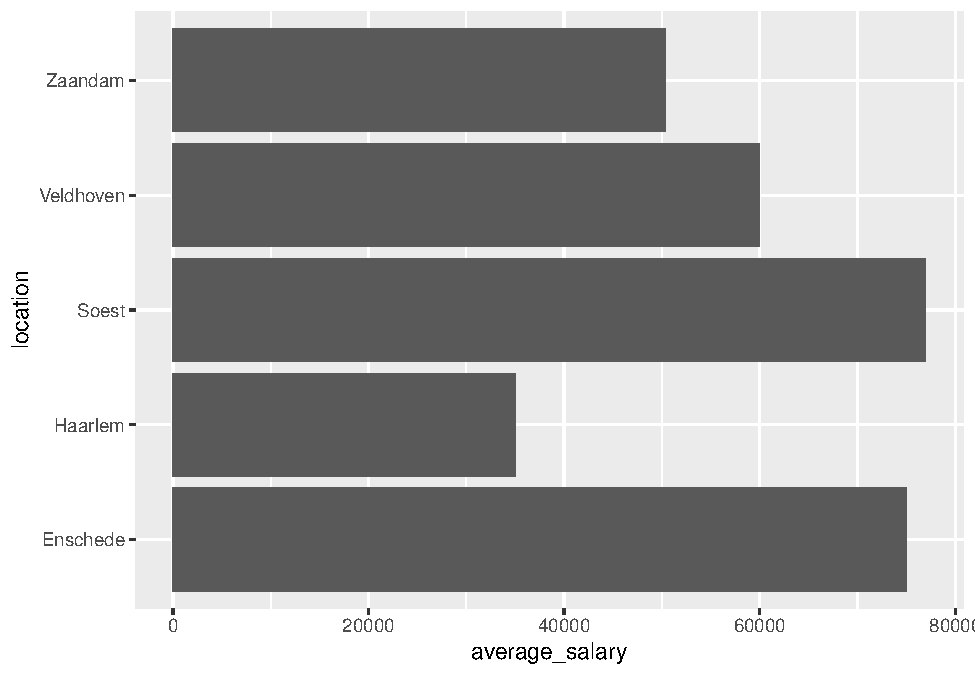
\includegraphics{analysis_files/figure-latex/unnamed-chunk-35-1.pdf} 6.2
top locations in terms of salary for data scientists

\begin{verbatim}
## [1] 4
\end{verbatim}

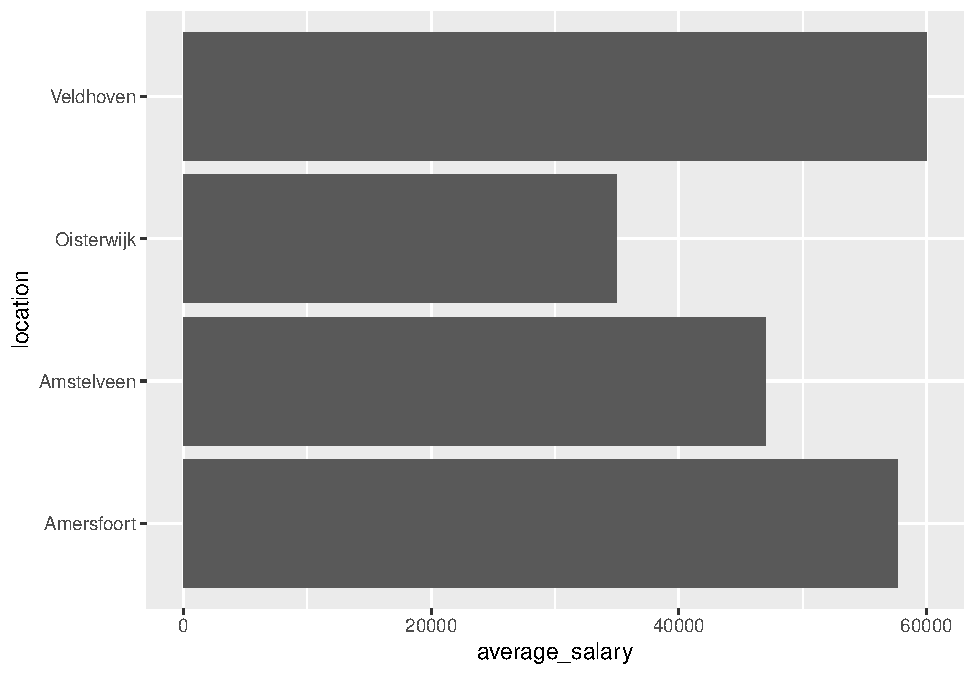
\includegraphics{analysis_files/figure-latex/unnamed-chunk-36-1.pdf} 6.3
top locations in terms of salary for data analysts

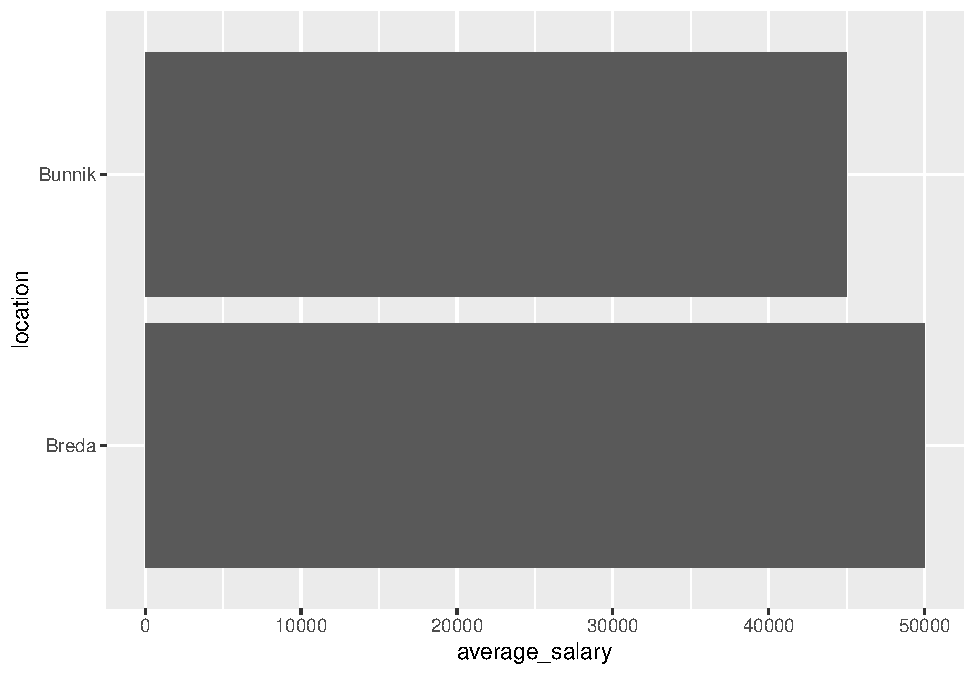
\includegraphics{analysis_files/figure-latex/unnamed-chunk-37-1.pdf}

6.4 top locations in terms of salary for marketing analysts

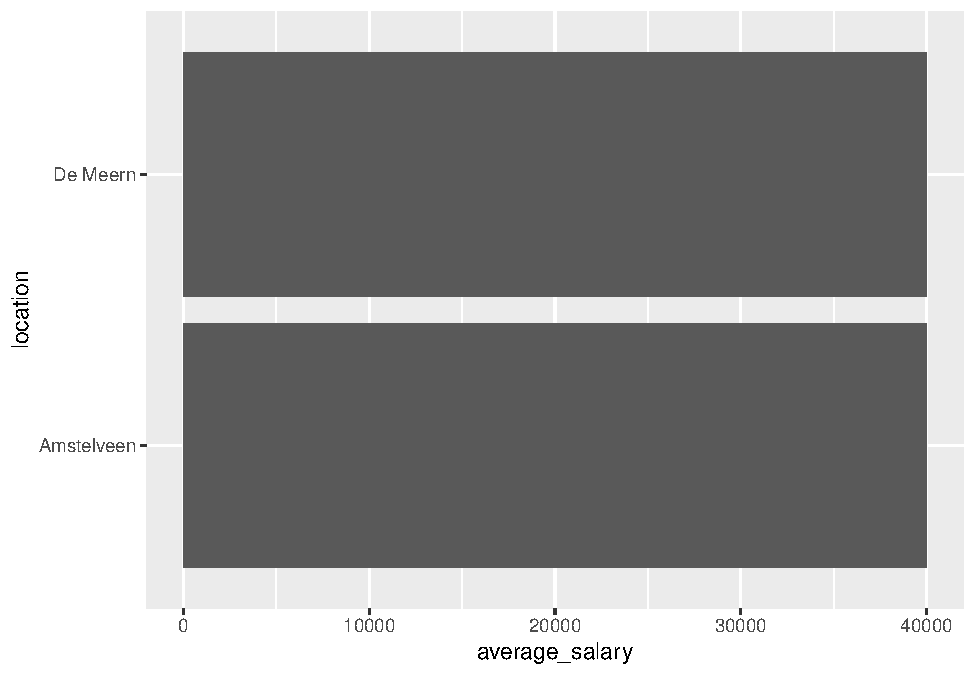
\includegraphics{analysis_files/figure-latex/unnamed-chunk-38-1.pdf} 6.5
top locations in terms of salary for marketeers

\begin{verbatim}
## Warning in merge.data.frame(salary, marketing_analist_avgsalary, by =
## "location"): column names 'average_salary.x', 'average_salary.y' are duplicated
## in the result
\end{verbatim}

\includegraphics{analysis_files/figure-latex/unnamed-chunk-39-1.pdf}

\begin{verbatim}
## here() starts at C:/Documents/data1/indeed-job-listings
\end{verbatim}

\begin{verbatim}
## pdf 
##   2
\end{verbatim}

\begin{verbatim}
## pdf 
##   2
\end{verbatim}

\begin{verbatim}
## pdf 
##   2
\end{verbatim}

\begin{verbatim}
## pdf 
##   2
\end{verbatim}

\begin{verbatim}
## pdf 
##   2
\end{verbatim}

\begin{verbatim}
## pdf 
##   2
\end{verbatim}

\begin{verbatim}
## pdf 
##   2
\end{verbatim}

\begin{verbatim}
## pdf 
##   2
\end{verbatim}

\begin{verbatim}
## pdf 
##   2
\end{verbatim}

\begin{verbatim}
## pdf 
##   2
\end{verbatim}

\begin{verbatim}
## pdf 
##   2
\end{verbatim}

\begin{verbatim}
## pdf 
##   2
\end{verbatim}

\begin{verbatim}
## pdf 
##   2
\end{verbatim}

\begin{verbatim}
## pdf 
##   2
\end{verbatim}

\begin{verbatim}
## pdf 
##   2
\end{verbatim}

\begin{verbatim}
## pdf 
##   2
\end{verbatim}

6.6 Getting insights into comparing the salaries of the 4 job titles on
the best locations

This plot shos that data sientists in general dominate salaries in each
location, shortly followed by data analist and marketing analist.
However, in Leiden, there seems to be a particularly attractive
marketing analist position opening up.

7 conclusion and discussion

7.1 Conclusion

Our results show that the main skills required by jobs related to Data
analysis, Data Science and Marketing are Excel, SQL, R and Python. The
curriculum of Marketing Analytics is focused more on R and SPSS, and
completely ignores SQL. We believe that students would benefit from the
inclusion of courses which develop skills in SQL and Python.

For location, Amsterdam is the clear winner when it comes to number of
job offers for any of our 4 search terms. Utrecht comes in 2nd and
Rotterdam, Den Haag and Eindhoven make up the top 5. The results make
sense since this are also the biggest cities in terms of population
within the Netherlands. The results were pretty similar for the 3 data
jobs but we saw a clear difference for marketeer jobs, where relatively
more opportunities were situatied outside of the Randstad in cities such
as Nijmegen, Breda and Arnhem. For salary, data scientist seem to be in
the best position, with on average the highest salaries compared to
marketeers, data analysts and marketing analysts.

7.2 Discussion

Our research is limited due to limited sample size. Scraping indeed had
its fair share of challenges and our focus on the Netherlands meant that
we collected between 500 and 1100 observations per job search. However
after cleaning out duplicates these numbers got adjusted downward.
Especially for the salary analysis, there was a lot of missing data
which meant datasets with a few hundred observations. This means that
some of the location averages for salary could be very high or very low
due to only one job being offered in that location with perhaps a very
high or very low salary. THis suggests that the salary analysis is
sensitive to outlier datapoints. This limited sample is however
difficult to overcome, since most job ads do not show salary data.

7.3 Future research Our results can be reproduced for any job title and
any location in the world. This makes it very interesting for future
research to compare different countries with eachother in terms of
salary and job skills for the 4 jobs researched in this analysis.
However, it also opens up the opportunity to students and job seekers in
general perform similar research in any kind of other field they are
interested in. By tweaking the search term in the scraper and the skills
being asked in the keyword analysis, it is possible to research for
example what skills are important in a range of jobs and locations.
Furthermore, we think that our analysis could be valuable over time by
for example repeating the research on a monthly or yearly basis to
observe possible developments over time in skills required, salaries
offered and locations offering the most jobs.

\end{document}
